%%%%%%%%%%%%%%%%%%%%%%%%%%%%%%%%%%%%%%%%%%%%%%%%%%%%%%
%\section{Human Activity Recognition}
%%%%%%%%%%%%%%%%%%%%%%%%%%%%%%%%%%%%%%%%%%%%%%%%%%%%%%
\label{sec:HAR}

\newcommand{\IR}{\mathbb{R}}

In this section we describe the implementation of the human activity
recognition ('HAR') component on the mobile device.  The algorithmic
foundations of this data mining task have been described in detail in
deliverable D2.2 in section 3.2 ``Mobile Sensing and activity
recognition''. We include a brief summary here (\ref{sec:har_method})
for the sake of completeness. Subsection \ref{sec:har_component}
contains the descriptions of the implementation. In subsection
\ref{sec:har_eval} we evaluate our method on two data sets and compare
it to the state of the art approaches.

\subsection{HAR Method Summary}\label{sec:har_method}

The process of activity recognition uses a pipeline of signal
processing and machine learning techniques. It consists of two phases:
the ``training phase'' and the ``integration phase''. 

\begin{figure}[htbp]
\centering
\subfigure[HAR Training Phase]{
\label{fig:har_overview}
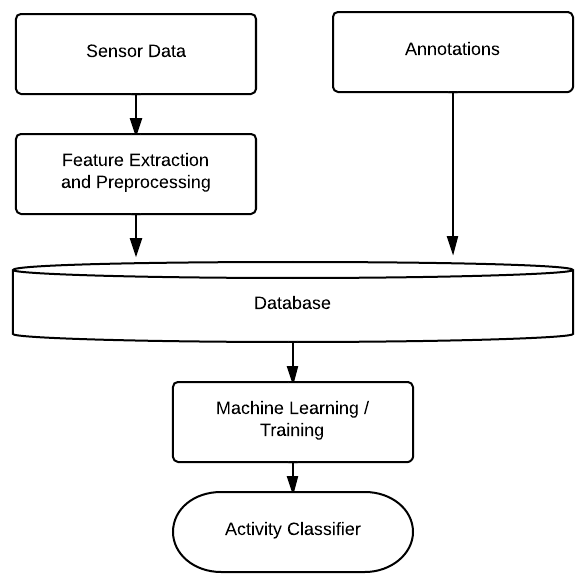
\includegraphics[width=0.45 \textwidth]{img/har/classification_overview.png}
} \hspace{1cm}
\subfigure[HAR Integration Phase]{
\label{fig:integrated_har_overview}
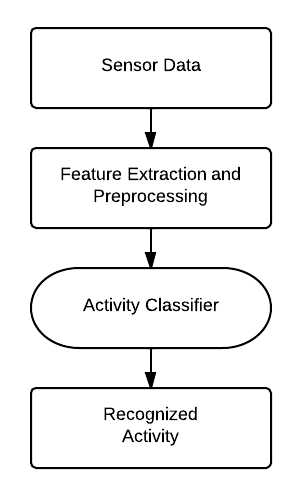
\includegraphics[width=0.25 \textwidth]{img/har/integration_overview.png}
}
\caption{Human Activity Recognition Method Overview}
\label{fig:HAR_PHASES}
\end{figure}

In the training phase (cf. Figure \ref{fig:har_overview}) a group of
volunteers is asked to perform the targeted activities for a certain
amount of time, while recording sensor samples with the device in
their pocket.  The gained training data stored in a database and used
to train a classifier of the activities.

In the integration phase (cf. \ref{fig:integrated_har_overview}), the
trained classifier is embedded into the mobile device.

Both phases rely on the preprocessing steps of "windowing'' and
``feature generation''. The stream of incoming sensor data is divided into
time windows of fixed size (typically 1-10 sec.) and for each window
a set of features is computed. This features are filtering out
relevant information from the raw signal. Typical features include
mean values and standard deviations as well as frequency domain
features like Fourier modes.

Deliverable D2.2 contains detailed lists of all sensors and features
and data mining methods that are used in the literature as well as
discussions of quality of the recognition results.

\subsection{Component Description}\label{sec:har_component}

The Human Activity Recognition Component implements the two phases
described in Figure \ref{fig:HAR_PHASES}. The training phase is
executed offline on a server and uses the following processing
pipeline (cf. Figure \ref{fig:classification_architecture}).

\begin{figure}[htbp]
\centering
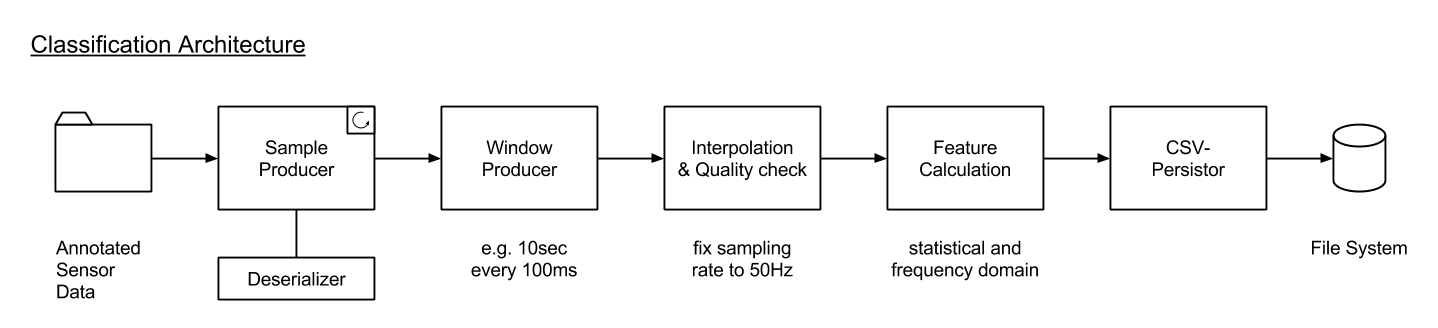
\includegraphics[width=\textwidth]{img/har/classification_architecture.png}
\caption{HAR Training Pipeline}\label{fig:classification_architecture}
\end{figure}

\begin{enumerate}
  \item {\bf Annotated Sensor Data.} The training data is stored as
    ssf files in the file system. The annotations are represented as
    folder structure. In this way it becomes very easy to add new
    training data to the repository. Using the inspection web tool,
    one can select appropriate time slices and export the
    corresponding samples as ``.ssf'' file. The exported file is then
    moved to the folder corresponding to the recorded activity.
  \item {\bf Sample Producer.} The sample producer service reads the 
    sensor samples from the file system and pushes them onto a generic 
    sample processing pipeline. The interface is designed a way that
    resembles the incoming data stream on the mobile device.
  \item {\bf Window Producer.} The window producer takes as
    constructor parameters a window-length and a delay. Incoming
    sensor samples are grouped in windows of the given length and
    passed further down as a single object.
  \item {\bf Interpolation and Quality Check.}  
    The recorded sensor data can be subject so several irregularities,
    like frequency disparities or small outtakes. To ensure that those
    irregularities do not pollute the training data we perform quality
    checks on the individual windows and interpolate the samples to a
    constant frequency of $50Hz$.
  \item {\bf Feature Calculation.} The classification calculates
    different features extracted from windows of raw sampling data. A
    description of the used features is included in section
    \ref{sec:feature_calc}.
  \item {\bf CSV-Persistor.} The calculated feature vectors are stored
    on the file system as CSV file. 
\end{enumerate}

In the next step the stored annotated feature vectors are used for
training of machine learning classifiers. For this task we relyed on 
available external tools like
WEKA\footnote{\url{http://www.cs.waikato.ac.nz/ml/weka/}}
and libsvm\footnote{\url{http://www.csie.ntu.edu.tw/~cjlin/libsvm/}}.
More details of the classification methods are given in section
\ref{sec:har_classifier_training}.
The trained classifiers were then exported as java methods and
integrated into the mobile HAR service (cf. Figure \ref{fig:integrated_har}).

\begin{figure}[htbp]
\centering
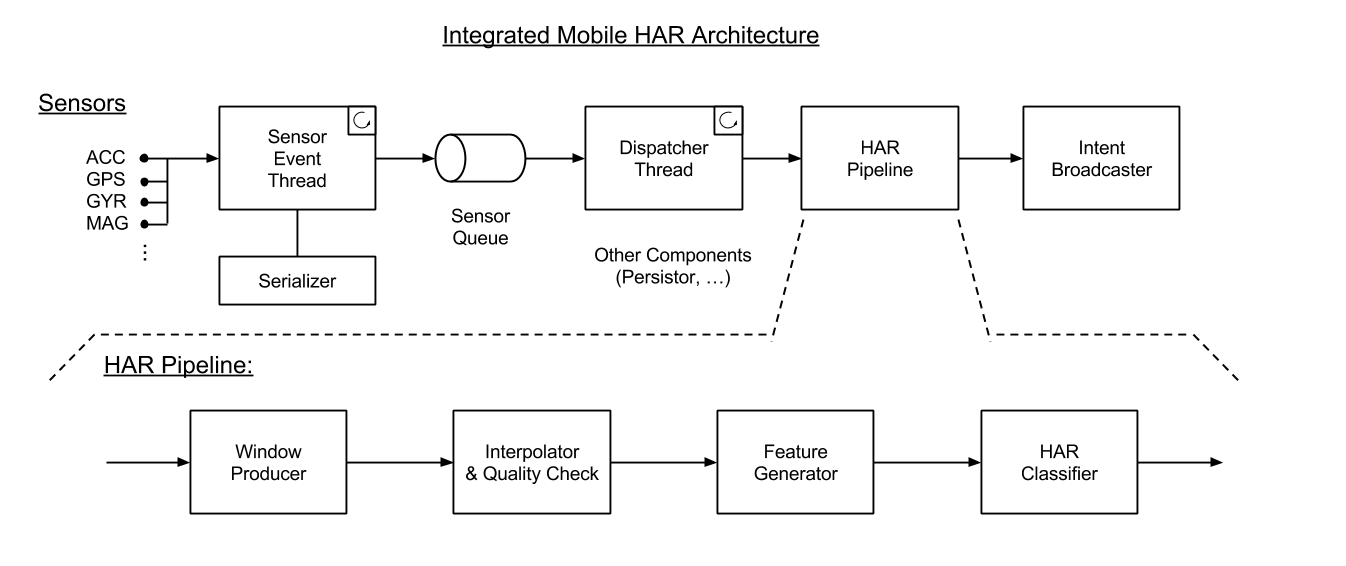
\includegraphics[width=\textwidth]{img/har/integration.png}
\caption{Integrated HAR Architecture}\label{fig:integrated_har}
\end{figure}

The integrated mobile HAR architecture consists of the following components.
\begin{enumerate}
\item {\bf Dispatcher Thread.} The dispatcher thread is part of
  the sensor collection architecture described in Chapter
  \ref{chap:sc}. It emits all gathered samples in the ssf format.
\item {\bf HAR Pipeline.} The HAR pipeline reuses most parts described
  in Figure \ref{fig:classification_architecture}. The Sample Producer
  is replaced by the Dispatcher Thread as source for sensor data.
\item {\bf HAR Classifier.} The HAR classifier component warps
  exported java method and outputs the results of the classification
  as string objects. The current implementation uses a decision tree.
\item {\bf Intent Broadcaster.} The classification results are
  broadcasted as an intent for use in other parts of the system
  (e.g. GUI, storage).
\end{enumerate}

\subsection{Feature Calculation}
\label{sec:feature_calc}

For the classifiaction of activities, we cannot directly use the raw
stream of sensor data. The reason is that machine learning classifiers
cannot operate on data streams directly, but need to get explicit
vectors as input. Moreover, these vectors cannot have arbitrary
dimension. If we feed in the raw sensor signal of only 5 seconds
recording, we get a vector of dimension
\[ d = 50 Hz \cdot 5 sec \cdot 3\ axes = 1000, \]
which is too much to handle for most classification algorithms.

With the calculation of features, we try to reduce the dimensionality
of the input signal, while keeping the essential information contained
in the signal. We use two different methods for feature calculation
{\it manual selection} and an automated {\it PCA} based feature set.

\subsubsection*{\bf Manually Selected Features}

The following manual features have been selected:

\begin{center}
\begin{tabular}{|r|l|p{11.5cm}|} \hline
Index & Name     & Description \\ \hline
0            & id       & User ID of the recorded samples \\ \hline
1            & tag      & Name of the recoded activity    \\ \hline
2            & xMean    & Mean values of the individual axes \\ 
3            & yMean    &             \\ 
4            & zMean    &             \\ \hline
5            & xVar     & Variance of the individual axes  \\ 
6            & yVar     &             \\ 
7            & zVar     &             \\ \hline
8            & s2Mean   & Mean value of the length of the acceleration
                          vector. \\ \hline
9            & s2Var    & Variance of the length of the acceleration
                          vector \\ \hline
10           & tilt     & Average tilting angle of the device towards
                          the vertical axes. \\ \hline
11           & energy   & Total energy of the recording.  \\ \hline
12           & kurtosis & Kurtosis\footnote{\url{http://en.wikipedia.org/wiki/Kurtosis}} 
                          measure of "peakedness" of the length of 
                          the acceleration vector. \\ \hline
13-24        & S2Bins   & Histogram over the length of the
                          acceleration vector. \\ \hline
25-37        & FFTBins  & Historgram over the absolute values of the
                          Fourier Modes of the length of the
                          acceleration vector. \\ \hline
\end{tabular}
\end{center}

Our feature list has been guided by the literature (cf. D1.2,
\cite{lara12}).  These consist of statistical features (mean and
variance), that are computed for each of the three axes as well as for
the length of the acceleration vector $s_2 = \sqrt{x^2 + y^2 + z^2}$.
An explicit tilt-feature has been included to allow better separation
of the ``sitting'' and ``standing'' classes.

We also include frequency domain features.  The ``energy'' feature
measures the total spectral
density\footnote{\url{http://en.wikipedia.org/wiki/Spectral_density}}
of the signal. Furthermore a set of histogram features measures the
energy of different Fourier modes of the signal. We have divided
energy spectrum into 10 equally distributed bins, covering roughly
95\% of the observed energy spectrum in the training data. Two more
bins added for outliers above and below the bin coverage.

\subsubsection*{\bf PCA Based Features}

There is a lot of freedom in the manual choice of feature vectors.
Moreover, it is not clear that the heuristically selected features
are able to separate the categories well. An automated way of
selecting features is provided by the {\it Principal Component
  Analysis} (PCA) method.\footnote{\url{http://en.wikipedia.org/wiki/Principal_component_analysis}}
This method selects a number of linear features that maximize 
variance of the resulting data. We use a reduced vector size of $266$
dimensions to keep $90\%$ of the variance in our data set.

\subsection{Classifier Training}\label{sec:har_classifier_training}

In this section we present more details about the employed machine
learning methods for human activity recognition. Both methods rely on
a training set of annotated feature vectors, and cannot be used
directly on the data-streams. As was explained in D2.1 the two
presented methods are the most popular approaches in the literature
and have led to good classification accuracies in earlier work.

\subsubsection*{{\bf Decision Tree HAR classifier}}
\label{sec:DectionTree}

A decision tree uses a hierarchy of simple binary decisions to
classify a feature vector into a set of given categories.  To be more
precise, let $x_\bullet = (x_1, \dots, x_n)$ a feature vector with numeric
feature values $x_i \in \IR$, and $C=\{c_1, \dots, c_N\}$ a set of
target categories. The individual decision rules $R_k$ are of the form
$(x_j \geq \alpha)$ or $(x_j \leq \alpha)$ for some index $j$ and
threshold value $\alpha \in \IR$.  A decision tree, organizes several
of those rules $R_k$ into a binary tree structure. The leaf nodes are
linked to the corresponding target categories. Figure
\ref{fig:decision_tree} shows an example of a tree with 9 decision
nodes and 4 categories.

\begin{figure}[h]
\centering
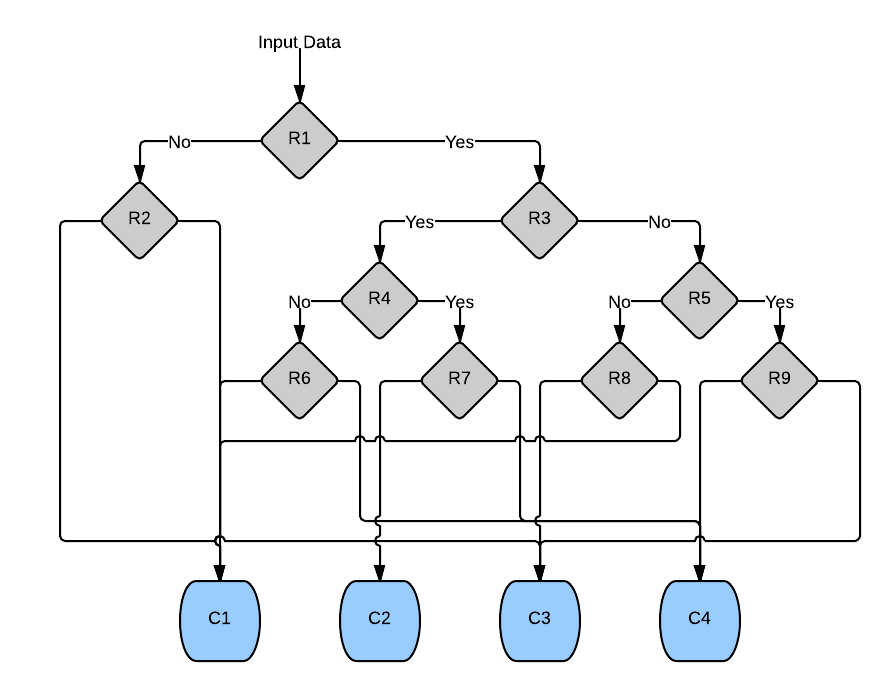
\includegraphics[width=0.5 \textwidth]{img/har/decision_tree.png}
\label{fig:decision_tree}
\caption{An example of a decision tree.}
\end{figure}

In the case of the activity recognition classifier, we have the
different activities (e.g. standing, walking, running) as 
categories and a set of manually computed features like (standard
deviations, or bin distributions of Fourier-modes) or automatically
generated PCA-based features to base our decision rules on.

Of course, we do not want to build a decision tree for the HAR task by
hand, but automatically learn a suitable tree on the basis of
annotated training data. For this task of decision tree learning,
several methods are known. Notable ones
include\footnote{\url{http://en.wikipedia.org/wiki/Decision_tree_learning}}:
ID3 (Iterative Dichotomiser 3), C4.5 (successor of ID3), CART
(Classification And Regression Tree), CHAID (CHi-squared Automatic
Interaction Detector).

We have chosen to use the C4.5 algorithm modified for continues
attribute values \cite{quinlan1996improved} since it has been
successfully used in the literature \cite{lara12} and an open source
implementation is available and integrated into the WEKA toolkit.

The C4.5 algorithm uses the concept of {\it information gain} to build
up a decision tree in a recursive, greedy fashion.  For a set of
annotated training vectors $T = \{ (x_\bullet, c) | c \in C \}$ a
decision rule $R$ splits $T$ into two subsets:
\[ T = T^+ \cup T^{-}, \quad T^+ = \{ R(x_\bullet, c) = \text{true}\}, \;
T^- = \{ R(x_\bullet, c) = \text{false} \} \]
The information gain of this rule is defined as 
\[ IG(T,R) = H(T) - \frac{|T^+|}{|T|} \cdot H(T^+) - \frac{|T^-|}{|T|} \cdot H(T^-), \]
where $H(S)$ is the entropy of the collection $S \subset T$
cf. \cite{Shannon1948}. The C4.5 algorithm finds the decision rule
with the largest information gain and uses this as the root for the
decision tree. It then recurses into the subset $T^+$ and $T^-$ and
adds the generated nodes as childs to the root node.

The choice of the threshold values $\alpha$ for the decision rules is
particularly crucial for the quality of the trained decision tee. A
possible improvement of the threshold selection algorithm can be
obtained by pre-clustering of the attribute values before the
training process cf. \cite{kotsiantis2006}.

Figure \ref{fig:dt_example} shows an example of a trained decision
tree on manually generated features.

\begin{figure}[h]
\tiny
\centering
\begin{verbatim}
J48 pruned tree
------------------

Number of Leaves  : 	52

Size of the tree : 	103


x18 <= 927
|   x24 <= 152
|   |   x20 <= 211
|   |   |   x4 <= -2.936108
|   |   |   |   x3 <= 1.132095
|   |   |   |   |   x18 <= 458
|   |   |   |   |   |   x35 <= 2: WALKING (6.0/1.0)
|   |   |   |   |   |   x35 > 2: CYCLING (2.0)
|   |   |   |   |   x18 > 458: SITTING (3.0)
|   |   |   |   x3 > 1.132095: CYCLING (527.0)
|   |   |   x4 > -2.936108
|   |   |   |   x4 <= 7.830095
|   |   |   |   |   x14 <= 13
|   |   |   |   |   |   x18 <= 87
|   |   |   |   |   |   |   x2 <= 3.434441
|   |   |   |   |   |   |   |   x3 <= -2.172633
|   |   |   |   |   |   |   |   |   x2 <= -3.51528: RUNNING (3.0/1.0)
|   |   |   |   |   |   |   |   |   x2 > -3.51528: WALKING (45.0/1.0)
|   |   |   |   |   |   |   |   x3 > -2.172633: CYCLING (5.0/1.0)
|   |   |   |   |   |   |   x2 > 3.434441
|   |   |   |   |   |   |   |   x19 <= 469: CYCLING (155.0)
|   |   |   |   |   |   |   |   x19 > 469: WALKING (4.0/1.0)
|   |   |   |   |   |   x18 > 87
|   |   |   |   |   |   |   x18 <= 415
|   |   |   |   |   |   |   |   x15 <= 17
|   |   |   |   |   |   |   |   |   x34 <= 60
|   |   |   |   |   |   |   |   |   |   x22 <= 138
|   |   |   |   |   |   |   |   |   |   |   x20 <= 98
|   |   |   |   |   |   |   |   |   |   |   |   x21 <= 58: CYCLING (10.0)
|   |   |   |   |   |   |   |   |   |   |   |   x21 > 58: WALKING (56.0)
|   |   |   |   |   |   |   |   |   |   |   x20 > 98
|   |   |   |   |   |   |   |   |   |   |   |   x17 <= 108

// TRUNCATED

x18 > 927
|   x10 <= 0.58851: SITTING (1071.0)
|   x10 > 0.58851
|   |   x3 <= -8.323328: WALKING (17.0)
|   |   x3 > -8.323328: CYCLING (15.0/2.0)
\end{verbatim}
\normalsize
\caption{Decision tree trained on manually computed features.}
\label{fig:dt_example}
\end{figure}

\subsubsection*{{\bf Support Vector Machine HAR Classifier}}
\label{sec:SVM}

A popular algorithm to train a binary classification model for mapping
features to activities is the Support Vector Machines (SVMs). SVMs are
known for their ability in smoothly generalizing and coping
efficiently with high-dimensionality pattern recognition
problems. They define a hypothesis space that includes all the
possible linear separations of the data
(Fig.~\ref{fig:svm_hypothesisSpace}) and they choose the one that
maximizes the margin between the two classes
(Fig.~\ref{fig:svm_margin}).

\begin{figure}[h]
\centering
  \includegraphics[width=0.5\textwidth]{img/svms/Svms_hypothesisSpace.pdf}
  \caption[Hypothesis spaces for SVM classifier.]{Left: Hypothesis space including all linear separations. Right: The selected hypothesis maximizes the margin.}
  \label{fig:svm_hypothesisSpace}
\end{figure}


\begin{figure}[h]
\centering
  \includegraphics[width=0.5\textwidth]{img/svms/Svm_Maxmargin.pdf}
  \caption{Maximization of the margin}
  \label{fig:svm_margin}
\end{figure}

\noindent The hyperplane that optimally separates the positive and the
negative class (i.e. maximizes the margin) can be described by
$\mathbf{w\cdot x + b = 0}$, where $\mathbf{w}$ is normal to the
hyperplane and $\frac{b}{\parallel\mathbf{w}\parallel}$ is the
perpendicular distance from the hyperplane to the origin
(Fig.~\ref{fig:svm_wb}). The optimal hyperplane can be obtained by
solving the following Quadratic Programming optimization problem:

\begin{equation}\label{Eq:svmQP0}
  \min \frac{1}{2}\parallel\mathbf{w}\parallel \quad \text{s.t.} \quad y_i(\mathbf{w}\cdot x_i + b) -1 \ge 0 \quad \forall i
\end{equation}

In order to relax the constraints of Eq.~\ref{Eq:svmQP0} and allow for
some misclassified points, a slack variable $\xi_i, i=1,\ldots,L$ is
introduced which transforms Eq.~\ref{Eq:svmQP0} into:

\begin{equation}\label{Eq:svmQPxi}
  \min \frac{1}{2}\parallel\mathbf{w}\parallel + C\sum_{i=1}^{L}\xi_i \quad \text{s.t.} \quad y_i(\mathbf{w}\cdot x_i + b) -1 +\xi_i \ge 0 \quad \forall i
\end{equation}

\noindent where the parameter $C$ controls the trade-off between the
slack variable penalty and the size of the margin. In the testing
phase, in order to classify an unseen example $x_t$, its distance to
the hyperplane is calculated using the formula $\mathbf{w}\cdot x_t +
b$. This distance indicates the classifier's confidence that the
unseen example $x_t$ belongs to the examined class.

\begin{figure}[h]
\centering
  \includegraphics[width=0.6\textwidth]{img/svms/Svms_wb.pdf}
  \caption{The resulting hyperplane after training an SVM.}
  \label{fig:svm_wb}
\end{figure}

The previous consider linear separation of the data. However, this is
rarely the case for most real world scenarios and for this reason the
kernel trick has been introduced. Applying the kernel trick to the
cases where the classes are not linearly separable in the input
feature space, we manage to map the features to a higher dimension
(Fig.~\ref{fig:svm_highDim}) where they can be linearly separated. For
example, in the case of an RBF kernel the otherwise linear hyperplane
is transformed to a hypersphere (Fig.~\ref{fig:svm_rbf}). For any
kernel $K(x,y)$, the classification model can be represented by a
vector $\textbf{w}$ (i.e. the model parameters), a bias scalar $b$ and
the support vectors $\mathbf{SV}_j, j=1,\ldots,N_{SV}$. For an unseen
example $x_t$, a confidence score is extracted by computing its
distance to the hyperplane of the model:

\begin{equation}\label{Eq:SVMdecision}
  confidence = \mathbf{w}*\sum_{j=1}^{N_{SV}}{K(\mathbf{SV}_j,\mathbf{x}_t)}+b
\end{equation}

\begin{figure}[h]
\centering
  \includegraphics[width=0.6\textwidth]{img/svms/Svm_DimensionMap.pdf}
  \caption{Illustration of the kernel trick for sample separation.}
  \label{fig:svm_highDim}
\end{figure}

\begin{figure}[h]
\centering
  \includegraphics[width=0.6\textwidth]{img/svms/Svm_RBF.pdf}
  \caption{Non-linear separation of the data using the RBF kernel}
  \label{fig:svm_rbf}
\end{figure}


In our case, an SVM model is trained on the previously extracted
features in order to learn the properties that define the examined
activity. The models are trained using the one versus all (OVA)
technique, i.e. all positive examples of the specific activity versus
all negative examples (i.e. the examples of all other activities). The
distance of a vector from the hyperplane indicates our confidence that
during the analysed window, the user performs the examined
activity. High positive values of this score increase our confidence
that this window belongs to the positive class while high negative
values provide strong confidence that the performed activity is not
the examined one.

% The fact that each model can be represented by a single vector and a
% scalar and that the testing process is essentially a vector
% multiplication, renders SVMs the best solution for a real time
% classification framework. This allows for storing the information
% about all the models in the phone memory, while testing is
% computationally very efficient, making it possible for the image
% classification algorithm to run entirely on a mobile phone.


\subsection{Evaluation}\label{sec:har_eval}

We have evaluated our classifier on two different datasets.

The first dataset was gathered on the University Campus in Koblenz in
December 2013.  It contains a total of around $900K$ samples collected
by $10$ volunteers.  The volunteers were instructed to perform the
activities ''walking'', ''running'', ''stairs'' and ''cycling'' on
predefined routes on the university campus. 
% (cf. Figure \ref{fig:data_collection_handout}). 
The total time effort per volunteer was about 20-25minutes and a financial reward was offered as
an incentive. After the recording the samples have been inspected
using our inspection tool and the beginning and ending of the
activities were manually stripped in order to avoid noise from holding
the device in the hand.

% \begin{figure}[htbp]
%   \centering
%   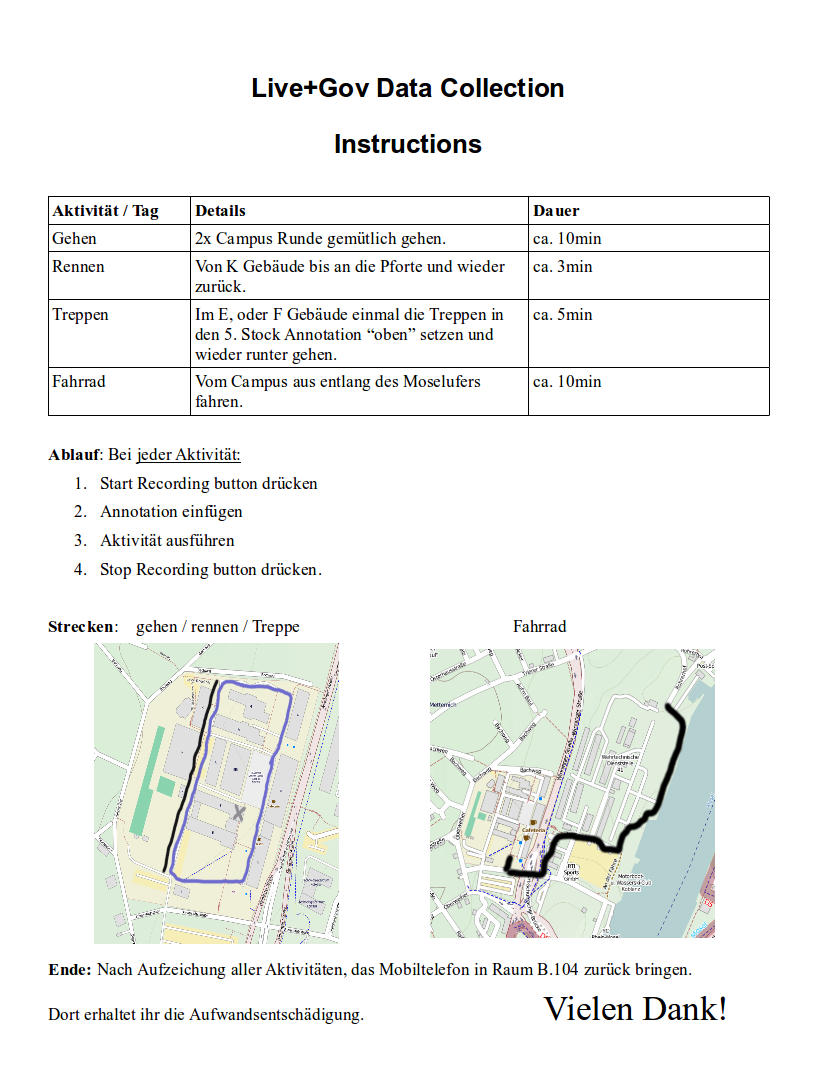
\includegraphics[width=\textwidth]{img/har/data_collection_handout.png}
%   \caption{Instructions for data collection in German
%     language}\label{fig:data_collection_handout}
% \end{figure}

The other dataset was obtained from the {\it UCI Machine Learning
  Repository}\footnote{\url{http://archive.ics.uci.edu/ml/datasets/Human+Activity+Recognition+Using+Smartphones}}
and was gathered by Davide Anguita, et. al. \cite{Anguita} in 2012.
It contains around $700K$ collected by 30 volunteers.

The number of samples per activity of both datasets are summarized in
Table \ref{fig:har_datasets}. Both datasets contain only
accelerometer samples, and have been preprocessed that have been
sampled at a fixed rate of $50Hz$.

\begin{table}[h]
\centering
\begin{tabular}{|l|r|r|} \hline
Activity  & UCI Dataset & UKOB Dataset \\ \hline
sitting   & 113.728     & 80.951        \\
standing  & 121.984     & 320.737       \\
walking   & 110.208     & 292.024       \\
running   & 0           & 31.916        \\
cycling   & 0           & 436.106       \\
stairs    & 188.800     & 30.086        \\
lying     & 124.416     & 0            \\ \hline \hline
Totals    & 659.136     & 903.156       \\ \hline
\end{tabular}
\caption{Number of accelerometer samples by activity and dataset.}
\label{fig:har_datasets}
\end{table}

Both datasets have been split into a training data-set and a test
data-set. The individual parts contain only full recordings of the
activities. No single recording is present in both parts of the
split. The volume is distributed in roughly $66/33$ ratio between
both parts.

We have three different parameters for the evaluation:
\begin{itemize}
\item {\bf Classifier.} Decision Tree (DT) or support vector machine (SVM)
\item {\bf Features.} Manually selected (MAN) or PCA based (PCA)
\item {\bf Dataset.} Self collected (UKOB) ore reference dataset (UCI)
\end{itemize}

We get the following evaluation results:
\begin{center}
\begin{tabular}{|lll|r|} \hline
  {\bf Classifier} & {\bf Features} & {\bf Dataset} & {\bf Accuracy in \%} \\ \hline
  DT	& MAN	& UKOB	&	$62$ \\ 
  DT	& PCA	& UKOB	&	$45$\\ 
  SVM	& MAN	& UKOB	& 	$\mathbf{87}$\\ 
  SVM	& PCA	& UKOB	&	$54$\\
  DT	& MAN	& UCI	&	$83$ \\ 
  DT	& PCA	& UCI	&	$68$ \\ 
  SVM	& MAN	& UCI	& 	$\mathbf{ 85 }$ \\ 
  SVM	& PCA	& UCI	&	$64$ \\ \hline
\end{tabular}
\end{center}

Figure \ref{fig:har_eval} shows a plot of these accuracy values.
\begin{figure}[ht]
  \centering
  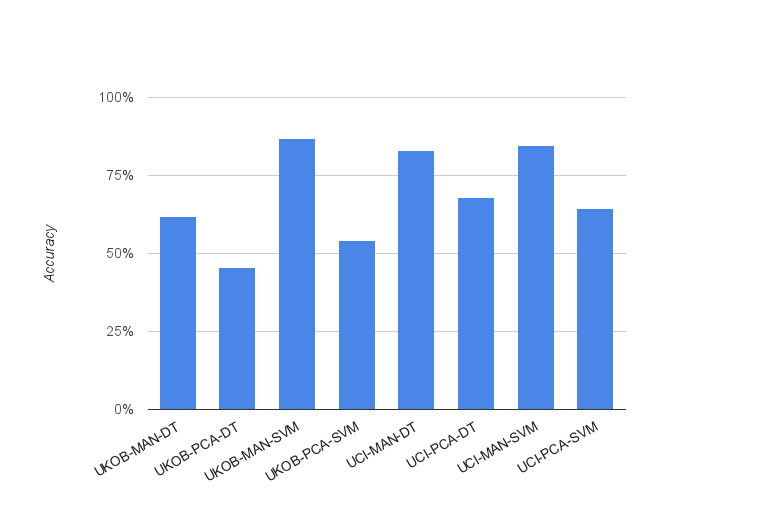
\includegraphics[width= 0.6 \textwidth]{img/har/accuracy_plot.png}
  \caption{Classification accuracy of HAR classifiers}
  \label{fig:har_eval}
\end{figure}

These figures show, that we are still around 10\% away from the state
of the art classifier used by \cite{Anguita} with 97\% accuracy. There
the authors use a multi-modal SVM on a similar list manually selected
feature vectors and slightly parameters for window length and overlap.
Our integrated application relies on a decision tree and manual
features, which show significantly weaker performance (64\%) than
state of the art in our experiments.

For both datasets the SVM trained on manual features performes best.
Although there are several parameters in the PCA feature extraction,
that remain to be optimized, the evaluation results suggest that
manually selected features yield better results.  For the UCI dataset
the decision tree is only slightly worse than the SVM based classifier
whereas the UKob dataset shows a more significant drop of
accuracy. This might be due to the fact that UKob dataset contains
slightly different activities than UCI, e.g. a large number samples is
recorded for the cycling activity, which is not present at UCI, and
conversely no samples for the lying task are present.

% Another anomaly is visible in the confusion matrices (cf. section
% \ref{sec:confusion_matrices}), is that we were not able to recognize
% the activity ``sitting'' in our own dataset. We do not currently have
% a good explanation of this anomaly. It points to structural problems
% in our approach, that need to be investigated further.

In conclusion, we have presented here a working HAR classification
architecture, that has been fully integrated into a mobile device and
has been evaluated against state of the art classifiers from the
literature on different datasets. Although the classification
accuracies are still behind state of the art, we are confident that we
can improve our methods exploiting the built up infrastructure.

% \clearpage
% \subsubsection{\bf Confusion Matrices}
% \label{sec:confusion_matrices}
% UCI-MAN-DT

\begin{tabular}{|l|rrrrrr|} \hline
Activitites & laying & sitting & stainding & walking & stairs down & stairs up\\
\hline
laying & 664 & 0 & 0 & 0 & 0 & 0\\
sitting & 0 & 542 & 64 & 0 & 0 & 0\\
standing & 0 & 135 & 521 & 0 & 0 & 0\\
walking & 0 & 0 & 0 & 1468 & 162 & 101\\
stairs down & 0 & 0 & 0 & 294 & 205 & 41\\
stairs up & 0 & 0 & 0 & 193 & 21 & 273\\
\hline
\end{tabular}

UKOB-MAN-DT

\begin{tabular}{|l|rrrrr|} \hline
Activities & cycling & running & sitting & stairs & walking\\
\hline
cycling & 1290 & 3 & 0 & 2 & 184\\
running & 0 & 30 & 0 & 0 & 29\\
sitting & 0 & 0 & 0 & 0 & 21\\
stairs & 15 & 0 & 1 & 92 & 127\\
walking & 142 & 11 & 0 & 812 & 784\\
\hline
\end{tabular}

UCI-PCA-DT

\begin{tabular}{|l|rrrr|} \hline
Activities & laying & sitting & standing & walking\\
\hline
laying & 664 & 0 & 0 & 0\\
sitting & 22 & 519 & 28 & 37\\
standing & 0 & 126 & 512 & 18\\
walking & 0 & 25 & 21 & 1685\\
\hline
\end{tabular}

UKOB-PCA-DT

\begin{tabular}{|l|rrrrr|} \hline
 & cycling & running & sitting & stairs & walking\\
\hline
cycling & 1051 & 64 & 1 & 1 & 362\\
running & 14 & 2 & 0 & 0 & 43\\
sitting & 747 & 0 & 0 & 0 & 32\\
stairs & 0 & 33 & 0 & 80 & 122\\
walking & 6 & 729 & 0 & 80 & 122\\
\hline
\end{tabular}

UKOB-MAN-SVM

\begin{tabular}{|l|rrrrr|} \hline
activities & cycling & running & sitting & stairs & walking\\
\hline
cycling & 1289 & 1 & 11 & 16 & 147\\
running & 0 & 59 & 0 & 0 & 0\\
sitting & 0 & 0 & 0 & 21 & 0\\
stairs & 12 & 0 & 0 & 75 & 140\\
walking & 57 & 0 & 1 & 60 & 1631\\
\hline
\end{tabular}

UCI-MAN-SVM

\begin{tabular}{|l|rrrrrr|} \hline
 & laying & sitting & standing & walking & stairs down & stairs up\\
\hline
laying & 664 & 0 & 0 & 0 & 0 & 0\\
sitting & 12 & 547 & 47 & 0 & 0 & 0\\
standing & 0 & 61 & 595 & 0 & 0 & 0\\
walking & 0 & 0 & 0 & 1642 & 71 & 18\\
stairs down & 0 & 3 & 0 & 291 & 230 & 16\\
stairs up & 0 & 0 & 0 & 185 & 15 & 287\\
\hline
\end{tabular}

UKOB-PCA-SVM

\begin{tabular}{|l|rrrrr|} \hline
 & cycling & running & sitting & stairs & walking\\
\hline
cycling & 1020 & 4 & 64 & 1 & 390\\
running & 38 & 0 & 0 & 0 & 21\\
sitting & 0 & 0 & 779 & 0 & 0\\
stairs & 203 & 1 & 0 & 3 & 28\\
walking & 1206 & 5 & 0 & 12 & 526\\
\hline
\end{tabular}

UCI-PCA-SVM

\begin{tabular}{|l|rrrrrr|} \hline
 & laying & sitting & standing & walking & stairs down & stairs up\\
\hline
laying & 664 & 0 & 0 & 0 & 0 & 0\\
sitting & 9 & 535 & 49 & 13 & 0 & 0\\
standing & 0 & 155 & 500 & 1 & 0 & 0\\
walking & 25 & 12 & 322 & 1307 & 32 & 33\\
stairs down & 21 & 2 & 79 & 432 & 5 & 1\\
stairs up & 6 & 1 & 31 & 432 & 7 & 10\\
\hline
\end{tabular}


%%% Local Variables:
%%% mode: latex
%%% TeX-master: "../D1-2"
%%% End:



%%% Local Variables:
%%% mode: latex
%%% TeX-master: "../D1-2"
%%% End:
